\documentclass[a4paper,12pt]{article}
\usepackage[a4paper, margin=2cm]{geometry}
\usepackage[utf8]{inputenc}
\usepackage{amsmath, amssymb} % Packages pour les maths
\usepackage[T1]{fontenc}
\usepackage{graphicx} 
\usepackage{caption}
\usepackage{setspace} % Espacement des lignes
\usepackage{tikz}
\usepackage{soul}

\usepackage{titlesec}
\usepackage{hyperref}
\renewcommand{\contentsname}{Table des matières}
\usepackage[colorlinks=true, linkcolor=blue, urlcolor=blue, citecolor=blue]{hyperref}
\titleformat*{\section}{\LARGE\bfseries}
\titleformat*{\subsection}{\Large\bfseries}
\titleformat*{\subsubsection}{\normalsize\bfseries}
\titleformat{\part}[display]
  {\normalfont\Huge\bfseries}{}{0pt}{}
\begin{document}
\begin{titlepage}
    \centering
    \vspace*{3cm}
    {\Huge \textbf{Document de Synthèse}\par}
    \vspace{2cm}
    {\Large Les Carcajous Callypiges\par}
    \vfill
    {\large 2025\par}
\end{titlepage}
\tableofcontents
\newpage
\addcontentsline{toc}{section}{Introduction}

{\LARGE \textbf{Introduction}}

\begin{center}
 \input{documentation/evolution_projet_1.txt}
\end{center}

  
  
\section{Modèle 1}
\subsection{Bille remplie d'eau}
\addcontentsline{toc}{subsubsection}{Hypothèses} 
\textbf{Hypothèses}

\begin{itemize}
    \item Terre assimilée à une boule d'eau, de température \(T_{\text{Terre}}\) telle que \(T_{\text{Terre}}\)> \(T_{\text{ext}}\)
    \item  Sans atmosphère (dans le vide)
    \item  Sans puissance solaire reçue  
    \item \(c_{m}= c_{\text{m,eau}} \sim c_{\text{m,Terre}}\) 
    \item $T(t=0) = T_i$ \ \ \
$T(t \to +\infty) = T_0$
   
\end{itemize}
$\rightarrow$ la terre perd de la température par rayonnement
\\ 

\addcontentsline{toc}{subsubsection}{Schéma}
\textbf{Schéma}
\\
\noindent\textcolor{gray}{\rule{\linewidth}{0.4pt}}

    
\begin{center}
  \input{modele1/figures/Schéma mathcha modèle 1.1.txt}
\end{center}



\noindent\textcolor{gray}{\rule{\linewidth}{0.4pt}} 

\vspace{1em}

\addcontentsline{toc}{subsubsection}{Equation}
\textbf{Equation}
\[   P = \sigma T^4 \cdot S
\]

\[    C \, \frac{dT}{dt} = - \sigma T^4 \,  \cdot S
\]

\[\frac{dT}{dt} = - \frac{4 \pi R_T^2 \sigma T^4}{C}\]  

Avec 
\(S= 4\pi r^2\)
\ \ \ \
\(\sigma=5,67 \cdot 10^{-8} W\cdot m^{-2} \cdot K^{-4}\)

\addcontentsline{toc}{subsubsection}{Solution}
\textbf{Solution} 
\[
T(t) = \left( \frac{C}{C/T_i^3 + 12\pi R^2 \sigma t} \right)^{1/3} 
= \frac{T_i}{\left(1 + 3k T_i^3 t \right)^{1/3}}
\]
avec \(k=\frac{4\pi R_T^2 \sigma}{C}\)
et \(C=c_{\text{m eau}}\times m=4,60 \cdot 10^{27} J\cdot K^{-1}\)

\bigskip



\bigskip

\addcontentsline{toc}{subsubsection}{Modélisation graphique}
\textbf{Modélisation graphique} 

\begin{center}
  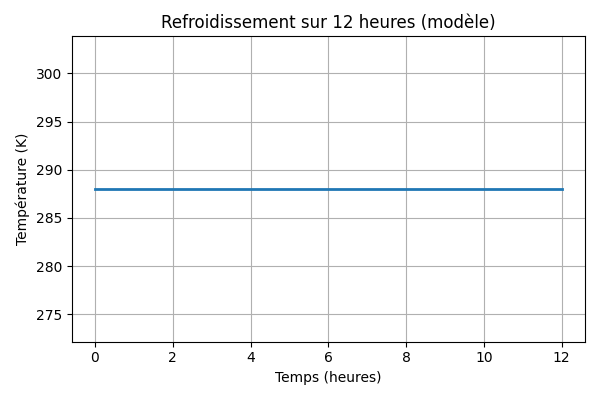
\includegraphics[width=0.8\linewidth]{../modele1/figures/modele1.png}
\end{center}
    
    

\subsection{Coquille vide }
\addcontentsline{toc}{subsubsection}{Hypothèses}
\textbf{Hypothèses}
\begin{itemize}
    \item On garde les hypothèses précédentes, excepté le système: la Terre est assimilée à une coquille d'eau, d'épaisseur dr, qui a un intérieur vide
    
\end{itemize}
$\rightarrow$ il faut donc recalculer la capacité thermique 

\addcontentsline{toc}{subsubsection}{Schéma}
\textbf{Schéma}

\noindent\textcolor{gray}{\rule{\linewidth}{0.4pt}}

    
\begin{center}
  \input{modele1/figures/Schéma modèle 1.2 coquille.txt}
\end{center}



\noindent\textcolor{gray}{\rule{\linewidth}{0.4pt}} 




\addcontentsline{toc}{subsubsection}{Calcul capacité thermique}
\textbf{Calcul capacité thermique}

\begin{align*}
m &= \rho_{\text{eau}} \left( \frac{4}{3} \pi (R_T + dr)^3 - \frac{4}{3} \pi R_T^3 \right) \\
&\overset{DL}{\approx} \rho_{\text{eau}} \cdot 4\pi R_T^2 \cdot dr \\
\\
C &= c_{\text{m,eau}} \cdot \rho_{\text{eau}} \cdot 4\pi R_T^2 \cdot dr \\
&= 4{,}31 \cdot 10^{20} \ \text{J} \cdot \text{K}^{-1} \\
\\
k &= \frac{\sigma }{c_{\text{eau}} \cdot \rho_{\text{eau}} \cdot dr}
\end{align*}
\vspace{0.5cm}
\subsubsection*{Modélisation graphique}   
\begin{center}
  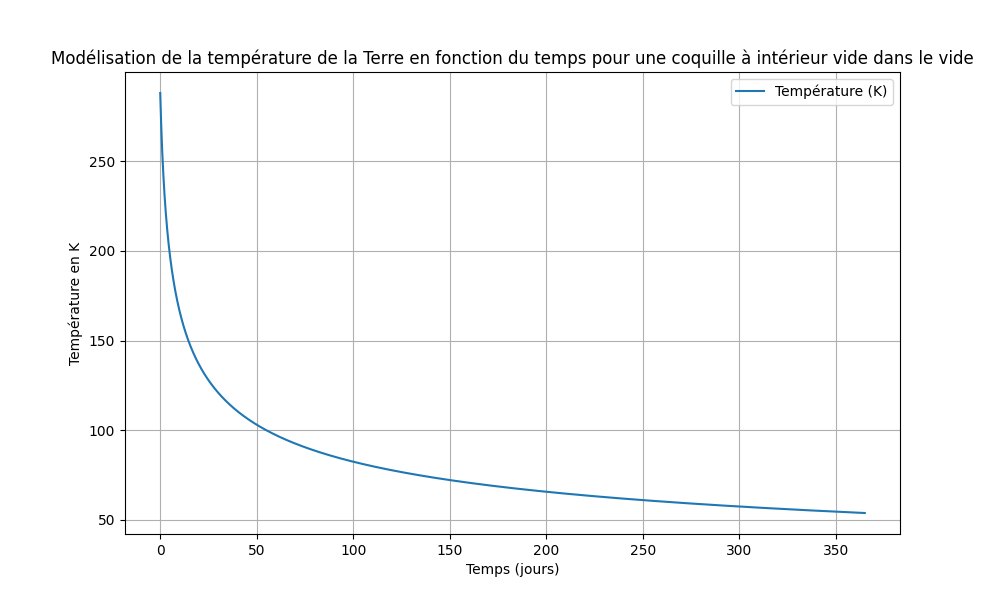
\includegraphics[width=0.8\linewidth]{../modele1/figures/modele1_coquille.png} 
\end{center}



\subsection{Critique du modèle}

\begin{itemize}
    \item Pas d’atmosphère, pas de rayonnement thermique reçu du Soleil, uniquement un transfert thermique émis par rayonnement.
    \item La Terre est assimilée à de d’eau.
    \item Température de la Terre subjective.
    \item Température du vide subjective.
    \item Épaisseur de la coquille arbitraire.
    \item On a supposé l'intérieur de la coquille vide, or cela implique un rayonnement à la fois vers l'intérieur et vers l'extérieur de la coquille.
\end{itemize}  

\newpage
\section{Modèle 2 : avec atmosphère}
\subsection{Boule d'eau avec atmosphère }
\addcontentsline{toc}{subsubsection}{Hypothèses}
\textbf{Hypothèses}
\begin{itemize}
    \item Terre assimilée à boule d'eau, de température \(T_{\text{Terre}}\) 
    \item  Atmosphère avec une température uniforme T 
    \item  Sans puissance solaire reçue  
    \item  Ignorance de la convection  
    \item \(c_m=c_{\text{m,Terre}}\sim c_{\text{m,eau}}\) 
    \item $T(t=0) = T_i$ \ \ \
$T(t \to +\infty) = T_0$
    \item La Terre ne rayonne pas
   
\end{itemize}
\vspace{0.5cm}
\subsubsection*{Schéma} 
\noindent\textcolor{gray}{\rule{\linewidth}{0.4pt}}

    
\begin{center}
  \input{modele2/figures/Schéma mathcha modèle 2.1.txt}
\end{center}
\noindent\textcolor{gray}{\rule{\linewidth}{0.4pt}}


\addcontentsline{toc}{subsubsection}{Équations de transfert thermique}
\textbf{Équations de transfert thermique}

On applique le premier principe au système \{ boule d'eau  \}

\begin{align*}
\delta Q &= C\, dT = -P_{\text{th,cond}} \cdot dt \\
\Rightarrow -\int \int \vec{j_{\text{th,cond}}}\, \vec{dS}\,dt = C\, dT \\
\Rightarrow -\int_{\theta=0}^\pi \int_{\phi=0}^{2\pi} h(T - T_0) \vec{e_{\text{r}}}\cdot r^2 \sin\theta\, d\theta\, d\varphi \vec{e_{\text{r}}}\, dt &=  C\, dT  \\
\Rightarrow -h(T - T_0) \cdot 4\pi\, dt &= C\, dT \\
\Rightarrow -T + T_0 = \frac{C}{h 4\pi} \frac{dT}{dt} \Rightarrow \frac{dT}{dt} &= -\frac{4\pi h}{C}(T - T_0)
\end{align*}

\vspace{0.5cm}

\addcontentsline{toc}{subsubsection}{Solution}
\textbf{Solution} 
$T(t) = T_0 + (T_i - T_0)e^{-kt}$ \quad avec $k = \frac{4\pi h}{C}$
\\
\bigskip

\addcontentsline{toc}{subsubsection}{Modélisation graphique}
\textbf{Modélisation graphique}
\begin{center}
  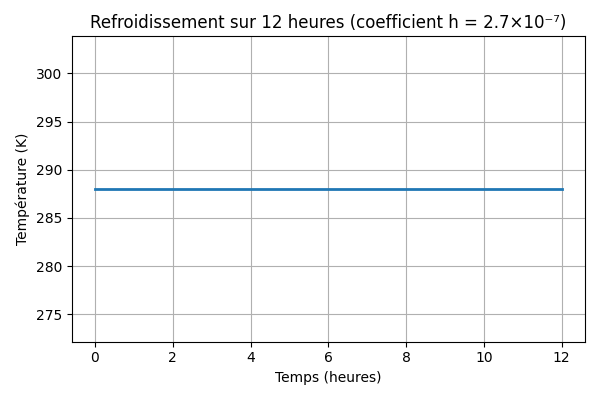
\includegraphics[width=0.8\linewidth]{../modele2/figures/modele2.png}
\end{center}
    
\vspace{1cm}
\subsection{Coquille assimilée à de l'eau avec atmosphère }
\addcontentsline{toc}{subsubsection}{Hypothèses}
\begin{itemize}
    \item On garde les hypothèses précédentes, en ajoutant l'atmosphère \end{itemize}
\vspace{1cm}
\addcontentsline{toc}{subsubsection}{Schéma}
\textbf{Schéma}
\\
\noindent\textcolor{gray}{\rule{\linewidth}{0.4pt}}

    
\begin{center}
  \input{modele2/figures/Schéma modèle 2.2 coquille.txt}
\end{center}
\noindent\textcolor{gray}{\rule{\linewidth}{0.4pt}}
\vspace{0.5cm}
\addcontentsline{toc}{subsubsection}{Modélisation graphique}
\textbf{Modélisation graphique}
\begin{center}
  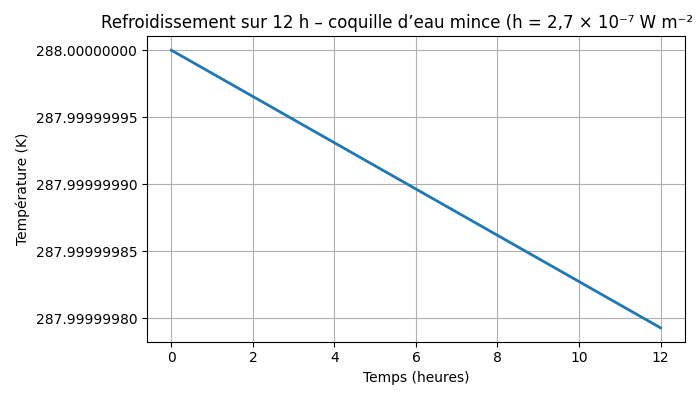
\includegraphics[width=0.8\linewidth]{../modele2/figures/modele2_coquille.png}
\end{center}
        


\subsection{Critique du modèle}

\begin{itemize}
    \item Température de la Terre subjective.
    \item Épaisseur de la coquille.
    \item Prise en compte de l’atmosphère donc utilisation de la loi de Newton :
    \begin{itemize}
        \item MAIS problème de définition de la couche limite puisqu’on ne souhaite pas prendre en compte la convection pour le moment.
    \end{itemize}
    \item Dans les codes \texttt{modele2\_coquille.py} et \texttt{modele2\_boule.py}, on a posé $h = \lambda_{\text{air}} / \delta$ avec $\lambda_{\text{air}} = 0{,}027 \, \mathrm{W/(K \cdot m)}$.
    \begin{itemize}
        \item On a pris $\delta = 100\, \mathrm{km}$ comme longueur de la couche limite pour ne pas se préoccuper de la convection avant la thermosphère (85 km – 600 km).
        \item Mais cette hypothèse ne semble pas pertinente, puisque la loi de Newton est adaptée à un modèle conducto-convectif.
        \item On peut donc prendre un $\delta$ plus raisonnable, de l’ordre de 50 cm.
    \end{itemize}
    \item Problème de définition de $T_0$ :
    \begin{itemize}
        \item Si on suit notre modèle, ce serait la température au-delà de la thermosphère.
        \item Or on a posé $T_0 = 273\, \mathrm{K}$ dans nos codes Python.
    \end{itemize}
\end{itemize}

\newpage
\section{Modèle 3 : intérieur de la coquille non vide }
\addcontentsline{toc}{subsubsection}{Hypothèses}
\textbf{Hypothèses}
\begin{itemize}
    \item Terre assimilée à une coquille d'eau avec intérieur non vide 
    \item  conduction entre centre de la terre et croûte (\(P_r\))
    \item  conduction entre croûte et air (\(P_{th,cond}\))
    \item  rayonnement de la croûte (\(P_{th,ray}\))
    \item On néglige le rayonnement de l'atmosphère
    \item $T(t=0) = T_i$ \ \ \
$T(t \to +\infty) = T_0$
     
\end{itemize}

\vspace{0.5cm}
\addcontentsline{toc}{subsubsection}{Schéma}
\textbf{Schéma}
\\
\noindent\textcolor{gray}{\rule{\linewidth}{0.4pt}}

    
\begin{center}
  \input{modele3/figures/Schéma modèle 3 coquille.txt}
\end{center}
\noindent\textcolor{gray}{\rule{\linewidth}{0.4pt}}

\addcontentsline{toc}{subsubsection}{Équations de transfert thermique}
\textbf{Équations de transfert thermique}

On applique le premier principe au système \{ coquille non vide  \}
\[
(-P_{\mathrm{th,cond}} - P_{\mathrm{th,ray}} + P_r)\,dt = C\,dT.
\]

\[
-\,h\bigl[T(r+dr)-T_0\bigr]\;4\pi
\;-\;4\pi\,\cdot (r+dr)^2\,\sigma\,T^4(r+dr)
\;-\;4\pi\,r^2\,\lambda\,\frac{\partial T}{\partial r}(r)
\;=\;C\,\frac{dT}{dt}.
\]

\medskip

Or au \(1^{er}\) ordre en \(dr\), \(r+dr\approx r\) :

\[
-4\pi\,h\bigl(T(r)-T_0\bigr)
\;-\;4\pi\,r^2\,\sigma\,T(r)^4
\;-\;4\pi\,r^2\,\lambda\,\frac{\partial T}{\partial r}(r)
\;=\;C\,\frac{dT}{dt}.
\]

\medskip

Avec
\[
P_{r}
= \iint\vec j_{\mathrm{thr}}\cdot d\vec S
= \iint -\lambda\,\vec{ \nabla } T\cdot d\vec S
= -\lambda
  \int_{0}^{\pi}\!\!\int_{0}^{2\pi}
    \frac{\partial T}{\partial r}\,\vec e_{r}\,
    r^2\sin\theta\;d\theta\,d\varphi\;\vec e_{r}
= -\lambda\,4\pi\,r^2\,\frac{\partial T}{\partial r}.
\]

\vspace{1cm}
\addcontentsline{toc}{subsubsection}{Modélisation graphique}
\textbf{Modélisation graphique}
    
    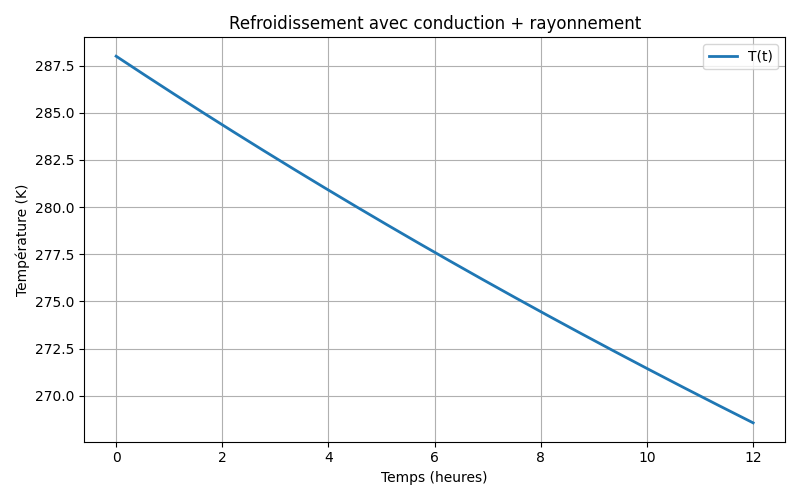
\includegraphics[width=0.8\linewidth]{../modele3/figures/modele3_coquille-conduction-rayonnement.png}    

\vspace{1cm}
\textbf{Critiques du modèle :}
\begin{itemize}
    \item La convection n’est pas prise en compte.
    \item dr doit être choisi de façon à ce que la température ne varie pas significativement.
    \item Problème de définition de $T_0$ :
    \begin{itemize}
        \item Si on suit notre modèle, ce serait la température au-delà de la thermosphère.
        \item Or on a posé $T_0 = 273\, \mathrm{K}$ dans nos codes Python. 
    
    \end{itemize}
\end{itemize}
\section{Modèle 4: }
\addcontentsline{toc}{subsubsection}{Hypothèses}
\textbf{Hypothèses}

\begin{itemize}
    \item Terre modélisée avec les continents, les mers, les océans 
    \item  On néglige: 
    \begin{itemize}
        \item convection dans l'air
        \item la conduction entre centre de la terre et croûte
        \item la conduction entre croûte et air (\(P_{th,cond}\))
    \end{itemize} 
    \item  rayonnement de la croûte (\(P_{th,ray}\))
    \item On considère la température de l'atmosphère constante dans l'espace et  au cours du temps 
    \item On prend en compte l'albédo du sol en fonction de la position et du mois de l'année 
    \item On prend en compte l'albedo des nuages.
    \item la capacité thermique dépend de la localisation
    \item On considère $T(t=0) = T_i$ \  indépendant de l'espace  
    \item On prend en compte la chaleur latente considérée avec des constantes propres à chaque continent\\
    
    
    
    
\end{itemize}


\addcontentsline{toc}{subsubsection}{Schéma}
\textbf{Schéma}
\noindent\textcolor{gray}{\rule{\linewidth}{0.4pt}}

    
\begin{center}
  \input{modele4/figures/Schéma modèle 4.txt }
\end{center}
\noindent\textcolor{gray}{\rule{\linewidth}{0.4pt}}
\vspace{0.2cm}
\addcontentsline{toc}{subsubsection}{Équations de transfert thermique}
\textbf{Équations de transfert thermique}


On applique le premier principe appliqué au système \{ Un pavé de hauteur h, de surface S de la Terre \}
\ \ 
\[
c_s \frac{dT}{dt} =(1-A_1)(1-A_2)\varphi_s-\sigma T^4+\sigma T_{atm}^4-\varphi_{lat}
\]
Avec
\begin{itemize}
    \item \(c_s\) la capacité thermique surfacique en \(J\cdot K^{-1}\cdot m^{-2}\)
     \item  \(T\) la température du système en \(K\)
    \item \(A_1\) l'albédo des nuages (sans unité)
    \item \(A_2\) l'albédo du sol (sans unité)
    \item \(\varphi_s\) le flux solaire incident en \(W \cdot m^2\)
 \item \(\sigma\) la constante de Stefan-Boltzmann \(W \cdot m^{-2} \cdot K^{-4}\)
    \item \(T_\text{atm}\) la température de l'atmosphère en \(K\)    
    
    \item \(\varphi_{lat}\) le flux de chaleur latente émis par notre système en \(W \cdot m^2\)
\end{itemize}



\vspace{0.5cm}
\addcontentsline{toc}{subsubsection}{Tabulation de l'albédo de surface en fonction de la position}
\textbf{Tabulation de l'albédo de surface en fonction de la position}

Les données ont été récupérées sur les dossiers CSV du projet (groupe B)  de l'année précédente. Il s'agit de moyennes mensuelles tabulées pour chaque position sur Terre (latitude longitude)
\addcontentsline{toc}{subsubsection}{Tabulation de l'albédo des nuages}
\textbf{Tabulation de l'albédo des nuages}

Obtenu par différence de l'albédo de la terre lors de ciel clair et ciel nuageux.
Moyennes mensuelles tabulées sur 1 an (1 janvier 2024 à 1 janvier 2025)
\\
\\
Source \url{https://ceres-tool.larc.nasa.gov/ord-tool/jsp/EBAFTOA421Selection.jsp}
\\
\\
Lien du code : \url{https://github.com/pierrelouis-cmrt/CREPES/blob/main/archive/para_spaciaux/albedo/albedo_nuages_jour.py}

\subsubsection{Calculs capacités calorifiques en fonction de la composition des surfaces}
Données récoltées sur : 
\url{https://data.catds.fr/cpdc/Land_products/GRIDDED/L4SM/OPER/}
\\
\\
Lien du code: \url{https://github.com/pierrelouis-cmrt/CREPES/blob/main/ressources/Cp_humidity/ZZ_cp.py}

\begin{itemize}
    \item Moyenne faite sur une période de 1 an grâce à 12 données récoltées le matin et 12 données récoltées le soir 
    \item Les 12 données ont été prise à des périodes différentes sur l'année 
    \item La masse volumique de la Terre est approximée constante 
    \item Pour le \text{Groenland} et l’Antarctique  
\end{itemize}
\[
w = \frac{\rho_w \theta}{\rho_b (1 - \theta) + \rho_w \theta}
\]
Avec \(\theta\): le taux d'humidité en \(m^3\) d'eau par \(m^3\) de sol 
\[
c_p = c_{p,\text{sec}} + w (c_{p,\text{eau}} - c_{p,\text{sec}})
\]
Avec \(w\): la fraction massique d'eau 
\begin{table}[h!]
\centering
\begin{tabular}{ll}
\textbf{Constante} & \textbf{Valeur} \\
\hline
$c_{p,\text{sec}}$ & \SI{0.80}{\kilo\joule\per\kilogram\per\kelvin} \\
$c_{p,\text{eau}}$ & \SI{4.187}{\kilo\joule\per\kilogram\per\kelvin} \\
$\rho_b$ (sol) & \SI{1300}{\kilogram\per\cubic\metre} \\
$\rho_w$ (eau) & \SI{1000}{\kilogram\per\cubic\metre} \\
\end{tabular}
\caption*{Constantes utilisées pour le calcul de $c_p$}
\vspace{1cm}
\end{table}

Détail du calcul de \( c_s \) :\\
\begin{align*}
c_s &= \frac{C}{S} \\
\text{Or } S &= \frac{m}{\rho h} \\
\text{Donc } c_s &= \frac{C \rho h}{m} = c_p  \rho  h
\end{align*}

\hspace*{2cm}Avec \( C \) la capacité thermique

\vspace{1cm} % <- ajoute un espace vertical de 0.5 cm

h : profondeur à partir de laquelle la température reste constante (cf. exo 1, TD chap. 11 sur la diffusion thermique), pour des variations de température journalières comprises entre 273\,K (la nuit) et 293\,K (le jour).\\

On obtient \( h \approx 0{,}40\,\mathrm{m} \).\\

(On nous donnait le coefficient de diffusion thermique du sol \( D_{\text{sol}} = 6 \times 10^{-7} \,\mathrm{m}^2/\mathrm{s} \).)



\subsection*{Chaleur latente}


Le flux de chaleur latente correspond à la puissance surfacique positive(reçue) ou négative(fournie) afin d'évaporer ou de condenser l'eau de la surface de la Terre.
On découpe la Terre de plusieurs manières, par mers et océans, et par continents. 
On parle d'une moyenne faite par continents :
\begin{itemize}
    \item Les mers et océans : 108.8 $W/m^2$
    \item L'Asie : 28.8 $W/m^2$
    \item L'Afrique : 45.1 $W/m^2$
    \item L'Europe : 38.1 $W/m^2$
    \item L'Amérique du Nord : 36.5 $W/m^2$
    \item L'Amérique du Sud : 73.1 $W/m^2$
    \item L'Océanie : 31.9 $W/m^2$
\end{itemize}

On suppose que la pression atmosphérique de la Terre est constante à la surface. On applique le premier principe de la thermodynamique :

\vspace{1cm}
\begin{align*}
    dH &= \delta Q \\
    dm \, \Delta h_{\text{vap}} &= P_{th} \times dt \\
    Dm \, \Delta h_{\text{vap}} &= P_{th}
\end{align*}

Donc, 
\begin{align*}
    \phi _{lat} &= \frac{Dm}{S}\Delta h_{vap}\\
    \phi _{lat} &= \frac{m}{S\Delta t}\Delta h_{vap}\\
    \phi _{lat} &= \frac{\rho V}{S\Delta t}\Delta h_{vap}\\
    \phi _{lat} &= \frac{\rho S E_{vap} \Delta t}{S\Delta t}\Delta h_{vap}\\
\end{align*}
Avec $E_{vap}$ l'évaporation en $m/s$.

\begin{tabular}{|c|c|}
\hline
Continents & évaporation ($\mathrm{cm/year}$) \\
\hline
Europe & 49 \\
\hline
Amérique du Nord & 47 \\
\hline
Amérique du Sud & 94 \\
\hline
Afrique & 58 \\
\hline
Asie & 37 \\
\hline
Océanie & 41 \\
\hline
Océans & 140 \\
\hline
\end{tabular}
\\
\url{https://environmentofearth.wordpress.com/2008/03/11/water-balance/?utm_source=chatgpt.com}
\\
\\
On obtient donc:

\\
\begin{tabular}{|c|c|}
\hline
Continents & Flux de chaleur latente ($\mathrm{W/m^2}$) \\
\hline
Europe & 38.1 \\
\hline
Amérique du Nord & 36.5 \\
\hline
Amérique du Sud & 73.1 \\
\hline
Afrique & 45.1 \\
\hline
Asie & 28.8 \\
\hline
Océanie & 31.9 \\
\hline
Océans & 108.8 \\
\hline
\end{tabular}

\subsubsection*{Modélisation graphique  :} 
\begin{itemize}
    \item Planisphère représentant les capacités calorifiques: 
\end{itemize}
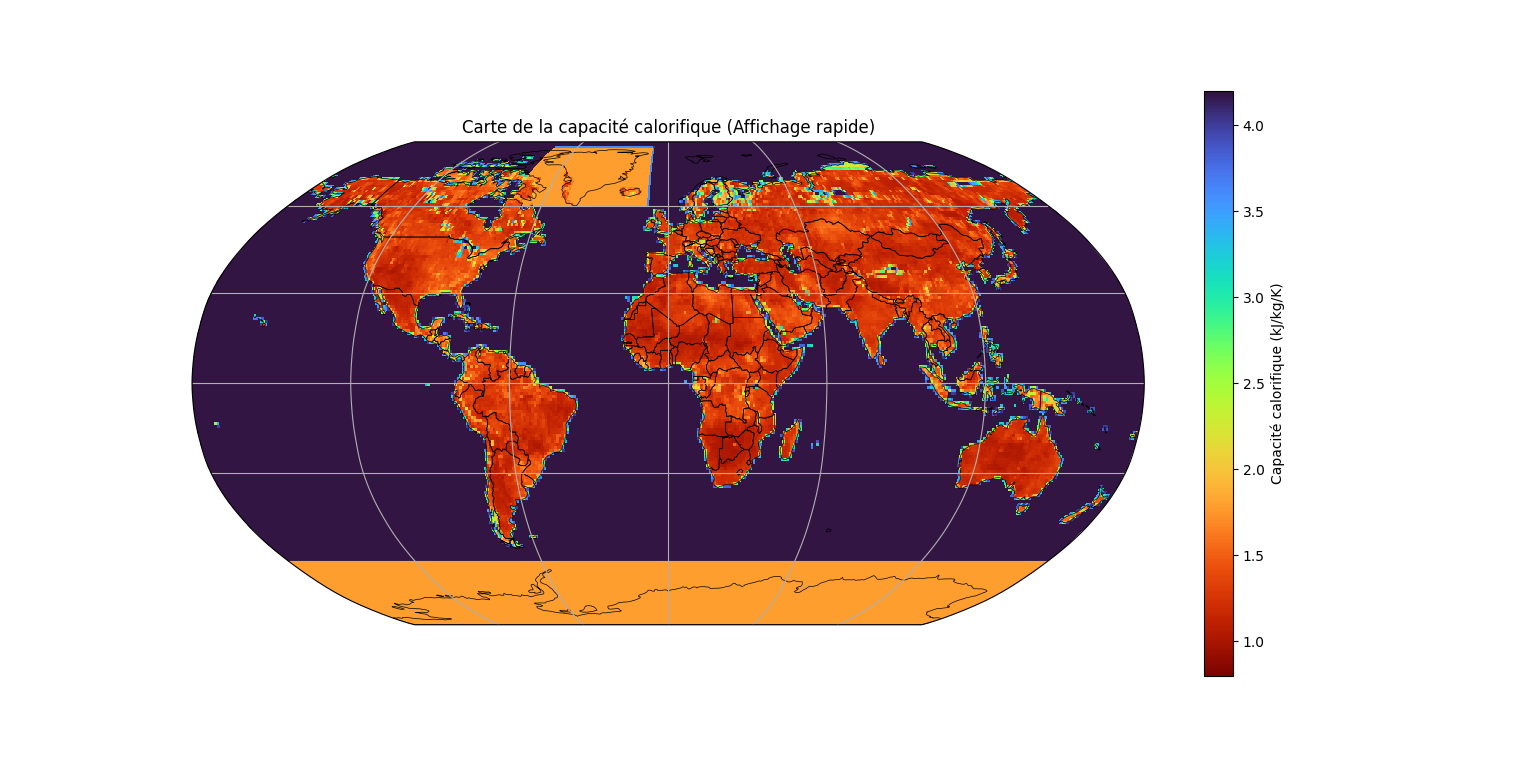
\includegraphics[width=0.8\linewidth]{modele4/figures/c_humidite.png}



\textbf{Critique du modèle}
\begin{itemize}
    \item On néglige la conducto-convexion
    \item On considère la température de l'atmosphère homogène et constante au cours du temps
    \item Les valeurs de chaleur latente sont prises constantes, ce qui n'est pas le cas en réalité
\end{itemize}
\end{document}